\chapter{系の設定}\label{chap:system}

この章では, 本研究で扱う系の設定について説明する. 

2次元の気液共存系で, 質量$m$の粒子が$N$個存在することを考え, 系の上下には壁, 左右には周期境界条件を課す. また, 重力を$y$軸負の向きにかけて, 熱流を$y$軸正の向きに流す. この熱流は, 系の上下の領域にそれぞれ異なる温度を設定したlangevin熱浴を使用することによってかけることとし, NVT-MDシミュレーションを実行する. また, 各熱浴の$y$幅は$8\sigma$となるように設定する. (図\ref{fig:system})


\begin{figure}[H]
  \centering
  \caption{系の概略図}
  \label{fig:system}
  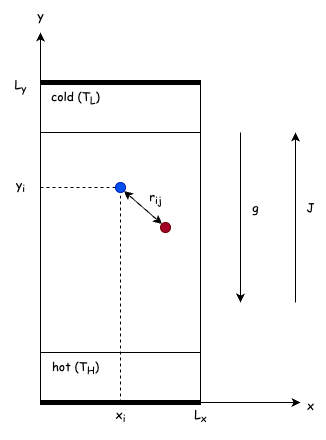
\includegraphics[scale=0.5]{image/system_pair.png}
\end{figure}

\section{ハミルトニアン}

\begin{align}
  \label{Hamiltonian}
  H(\Gamma; g)
  &= \sum_{i=1}^{N}
  \left[
    \frac{{\bm{p}_i}^2}{2m} 
    + \sum_{j > i}^{N}
      \tilde{\phi}_{\text{LJ}}^{\text{pair}}(r_{ij})
    + mgy_i
    + V^{\text{wall}} (y_i)
  \right] 
\end{align}

第1項から第4項まで順に, 運動エネルギー, 粒子-粒子間相互作用ポテンシャル, 重力ポテンシャル, 壁-粒子間相互作用ポテンシャルである. 以降, 本節では自明な運動エネルギーと重力ポテンシャルの項は別として, 第2項の粒子-粒子間相互作用ポテンシャル, 第4項の壁-粒子間相互作用ポテンシャルについて説明する.

\subsection{粒子-粒子間相互作用ポテンシャル}

シミュレーションを行う際に, 典型的な粒子間相互作用ポテンシャルとして, 12-6 Lennard-Jones Potential を採用する.

\begin{align}
  \phi_{\text{LJ}}^{\text{pair}}(r; \varepsilon, \sigma) = 4\varepsilon \qty[\qty(\frac{\sigma}{r})^{12} - \qty(\frac{\sigma}{r})^{6}] 
\end{align}

\begin{figure}
  \centering
  \caption{LJポテンシャル}
  \label{}
  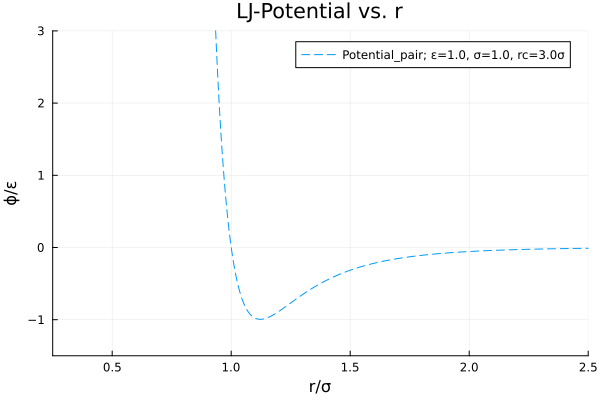
\includegraphics[scale=0.5]{image/LJ-Potential_pair.png}
\end{figure}

シミュレーション上では, カットオフ長 $r_{\text{cut}}^{\text{pair}}=3\sigma$ とポテンシャルのシフトアップを考慮して

\begin{align}
  \tilde{\phi}_{\text{LJ}}^{\text{pair}}(r;r_{\text{cut}}^{\text{pair}}) = \qty{\phi_{\text{LJ}}^{\text{pair}}(r) - \phi_{\text{LJ}}^{\text{pair}}(r_{\text{cut}}^{\text{pair}})}\theta \qty(r_{\text{cut}}^{\text{pair}}-r) \\
\end{align}

のように書き換えたポテンシャルを用いている.

\subsection{周期境界条件と最近接イメージ規約}

周期境界条件を考慮すると, 粒子-粒子間相互ポテンシャルの総計はまず以下のように書ける.\cite{MD}

\begin{align}
  \sum_{n_x \in \mathbb{Z}} \sum_{i=1}^{N} \sum_{\substack{j=1 \\ (j \neq i \ \text{for} \ n_{x} = 0)}}^{N} \frac{1}{2} \tilde{\phi}_{\text{LJ}}^{\text{pair}}(|\bm{r}_i -(\bm{r}_j + L_x \bm{e}_x)|) 
\end{align}

$n_x = 0$ (オリジナルセルの中)では, 同じ$i,\ j$ペアのポテンシャルエネルギーを2回足すことになるので, ポテンシャルを$1/2$している. その上で, $j = i$の場合は自分自身との相互作用になるため, これは除外する. $n_x \neq 0$の場合, 粒子$j$はイメージ粒子となるため, $j=i$の場合も含めることになる. このときにもダブルカウントがあるので, ポテンシャルを$1/2$している. 

\begin{figure}[H]
  \centering
  \caption{オリジナルセルとイメージセル}
  \label{fig:system_periodic}
  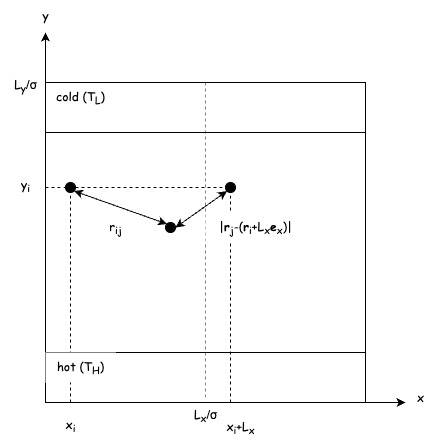
\includegraphics[scale=0.7]{image/system_periodic.jpg}
\end{figure}

注目する系の粒子が常にオリジナルセルの中にとどまっているかのようにMD上で扱うには,

\begin{align}
  x_{i} = x_{i}' \mod L_{x} 
\end{align}

と,  飛び出した粒子の$x$座標$x_{i}'$を上式のように$x_i$にシフトすれば良い. しかし, 周期境界条件とセットに, 最近接イメージ規約として, 粒子$i$がオリジナル粒子と各イメージ粒子の中で最も近い粒子$j$らとのみ相互作用をすることを課すと, 粒子間の相互ポテンシャルの総計は先ほどよりも簡単に書けるようになる.

\begin{align}
  \sum_{i=1}^{N} \sum_{j > i}^{N} \tilde{\phi}_{\text{LJ}}^{\text{pair}} (r_{ij})
\end{align}


\subsection{壁-粒子間相互作用ポテンシャル}

\begin{align}
  \phi_{\text{LJ}}^{\text{wall}}(r; \varepsilon^{\text{wall}}, \sigma^{\text{wall}}) = 4\varepsilon^{\text{wall}} \qty[\qty(\frac{\sigma^{\text{wall}}}{r})^{12} - \qty(\frac{\sigma^{\text{wall}}}{r})^{6} ] \\
\end{align}

各パラメータは以下のように設定する.

\begin{align}
  \varepsilon^{\text{wall}} &= \varepsilon \\
  \sigma^{\text{wall}} &= \qty(0.5 + \text{R}_\text{t}) \times \sigma \\
  r^{\text{wall}}_{\text{cut}} &= \qty(2^{1/6} + \text{R}_\text{a}) \times \sigma^{\text{wall}}
\end{align}

カットオフ長とシフトアップを考慮して

\begin{align}
  \tilde{\phi}_{\text{LJ}}^{\text{wall}}(r;r_{\text{cut}}^{\text{wall}}) = \qty{\phi_{\text{LJ}}^{\text{wall}}(r) - \phi_{\text{LJ}}^{\text{wall}}(r_{\text{cut}}^{\text{wall}})}\theta \qty(r_{\text{cut}}^{\text{wall}}-r) \\
\end{align}

この系では, $y=0$と$y=L_y$に壁がついている. よって, 壁ポテンシャルは

\begin{align}
  V^{\text{wall}}(y; L_y) &= \tilde{\phi}_{\text{LJ}}^{\text{wall}}(y;r_{\text{cut}}^{\text{wall}}) + \tilde{\phi}_{\text{LJ}}^{\text{wall}}(L_y - y;r_{\text{cut}}^{\text{wall}})
\end{align}

のように書ける. これまでのことを踏まえて, 系のハミルトニアンは式\eqref{Hamiltonian}のように書き表せる.

\begin{align}
    H(\Gamma; g)
    &= \sum_{i=1}^{N}
    \left[
      \frac{{\bm{p}_i}^2}{2m} 
      + \sum_{j > i}^{N}
        \tilde{\phi}_{\text{LJ}}^{\text{pair}}(r_{ij})
      + mgy_i +V^{\text{wall}}(y_i)
    \right] \ \tag*{\eqref{Hamiltonian}} 
\end{align}

\section{熱浴領域}\label{sec:heat_region}

系の両端に温度制御できるランジュバン熱浴を設計することによって, 熱流を実装することにする.

\begin{figure}[H]
  \centering
  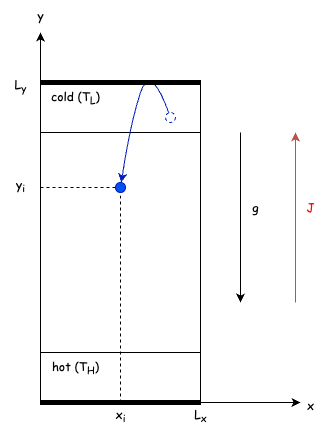
\includegraphics[scale=0.5]{image/system_heatflux.png}
  \caption{熱浴から飛び出る粒子の様子}
  \label{}
\end{figure}

粒子$i$が熱浴に侵入すると, その粒子の運動は以下のランジュバン方程式に従う. 

\begin{align}
  \label{langevin_r}
  \dot{\bm{r}_i} &= \pdv{H}{\bm{p}_i} \\
  \label{langevin_p}
  \dot{\bm{p}_i} &= - \pdv{H}{\bm{r}_i} - \gamma \dot{\bm{r}_i} + \sqrt{2 \gamma k_{\text{B}}T_{\nu}}\bm{\xi}_i (t) 
\end{align}

式\eqref{langevin_p}の第1項は速度に比例する抵抗力, 第2項はランダムな揺動力であり, $\bm{\xi}_{i}(t)$は以下の条件を満たすホワイトノイズである.

\begin{align}
  \bm{\xi}_{i}(t) &= ({\xi_{i}^{x}(t)}, {\xi_{i}^{y}(t)}, {\xi_{i}^{z}(t)}) \\
  \expval{\xi_{i}^{a}(t)} &= 0 \\
  \expval{\xi_{i}^{a}(t)\xi_{j}^{b}(t')} &= \delta_{i,j} \delta_{a,b}\delta (t-t')
\end{align}

また, 以下のように条件づけをしているので, 粒子がそれぞれの熱浴に侵入していないときには$\gamma=0$となり, 正準方程式に従うようになっている. 

\begin{align}
  \gamma(y_i) &= 1. \ T_{\nu}(y_i) = T_{\text{H}}. \ (0 < y_i < 8\sigma) \\
  \gamma(y_i) &= 1. \ T_{\nu}(y_i) = T_{\text{L}}. \ (L_y - 8\sigma < y_i < L_y) \\
  \gamma(y_i) &= 0.  \ (8\sigma < y_i < L_y - 8\sigma)
\end{align}

\section{重力と熱流を導入}

\ref{sec:heat_region}節において, $T_{\text{H}} < T_{\text{L}}$ として, 熱流が流れるようにする. 

当実験での系では, 熱流とともに重力ポテンシャルがかかっており, 重力と熱流のどちらも粒子密度の濃度勾配を生み出す効果をもつ. そこで両者の影響を比較するため, 系の上下両端のポテンシャルエネルギー差$mgL_y$と運動エネルギー差$k_{\text{B}}\Delta T \ (\Delta T \equiv T_{\text{H}} - T_{\text{L}})$の比を$\chi$として先行研究に倣って以下のように設定する. \cite{Yoshida}

\begin{align}
  \chi &\equiv \frac{k_{\text{B}}\Delta T}{mgL_{y}} = 1.265
\end{align}

\section{容器壁を系統的に比較}

壁の濡れ性を制御する無次元パラメータを2つ用意する.

\begin{align}
  \text{R}_\text{t} &: 壁の厚み. \\
  \text{R}_\text{a} &: 引力幅.
\end{align}

これらを用いて, 壁-粒子間相互作用のLJポテンシャルのパラメータ$\sigma^{\text{wall}}$と$r^{\text{wall}}_{\text{cut}}$を以下のように書き表す.

\begin{align}
  \sigma^{\text{wall}} &= \qty(0.5 + \text{R}_\text{t}) \times \sigma , \\
  r^{\text{wall}}_{\text{cut}} &= \qty(2^{1/6} + \text{R}_\text{a}) \times \sigma^{\text{wall}} 
\end{align}

パラメータ $(\text{R}_\text{t}, \text{R}_\text{a})$ を変えることによって, 壁-粒子間相互作用LJポテンシャルが変化する. このときに, 粒子集団の様相がどのように変わるのかをみることが本論の主題である.

$\text{R}_\text{t}$ と $\text{R}_\text{a}$ を少しずつ変えた系でシミュレーションをして, 粒子集団の様相の変化を見た. 以下に示すのが, それらを動かす範囲である.

\begin{align}
  \text{R}_\text{t} &\colon 0.0 \sim 0.5 \\
  \text{R}_\text{a} &\colon 0.0 \sim 3.0 - 2^{1/6} = 1.877538\dots
\end{align}

数値実験上で実際に入力する値を以下に示す. 本論では簡単のため小数点以下をいくらか簡略して示すことがある.

\begin{align}
  \text{R}_\text{t} &= 0.0,  0.125,  0.25,  0.375,  0.5 \\
  \text{R}_\text{a} &= 0.0,  0.4693845,  0.938769,  1.4081535,  1.877538
\end{align}

以下は$\text{R}_\text{t}$, $\text{R}_\text{a}$を変化させたときのLJポテンシャルがどのように変化するのかをそれぞれ可視化したグラフである.

参考のために, 各パラメータの値を変えることによって, カットオフ長と衝突直径がどのように変わるのかを示す.

\begin{align}
  \text{R}_\text{a} &= 0.0 \Rightarrow r_{\text{cut}}^{\text{wall}} = 2^{1/6} \sigma^{\text{wall}} \\
  \text{R}_\text{a} &= 1.877 \Rightarrow r_{\text{cut}}^{\text{wall}} = 3.0 \sigma^{\text{wall}} 
\end{align}

\begin{align}
  \text{R}_\text{t} &= 0.0 \Rightarrow \sigma^{\text{wall}} = 0.5 \sigma \\
  \text{R}_\text{t} &= 0.5 \Rightarrow \sigma^{\text{wall}} = \sigma 
\end{align}

である. 

\begin{figure}[H]
  \centering
  \begin{tabular}{ccccc}
    \begin{minipage}[t]{0.2\hsize}
      \centering
      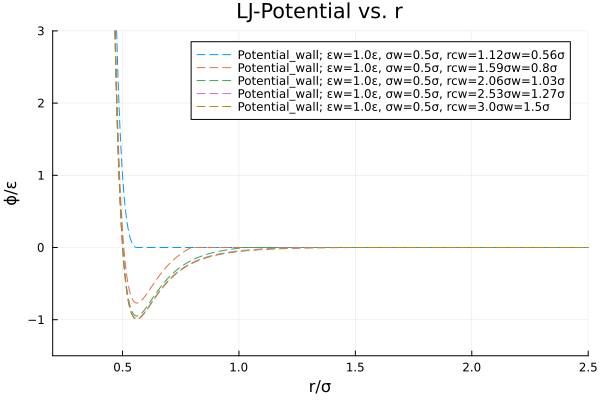
\includegraphics[width=\textwidth]{image/RaRtmap_LJ/LJ-Potential_Rt0.0.png}
      \subcaption{$\text{R}_\text{t}:0.0$}
      \label{}
    \end{minipage} &
    \begin{minipage}[t]{0.2\hsize}
      \centering
      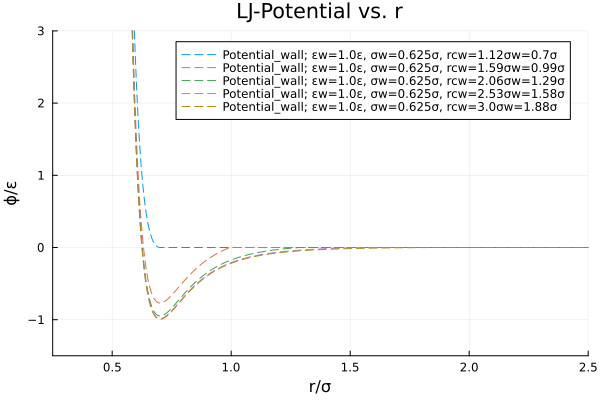
\includegraphics[width=\textwidth]{image/RaRtmap_LJ/LJ-Potential_Rt0.125.png}
      \subcaption{$\text{R}_\text{t}:0.125$}
      \label{}
    \end{minipage} &
    \begin{minipage}[t]{0.2\hsize}
      \centering
      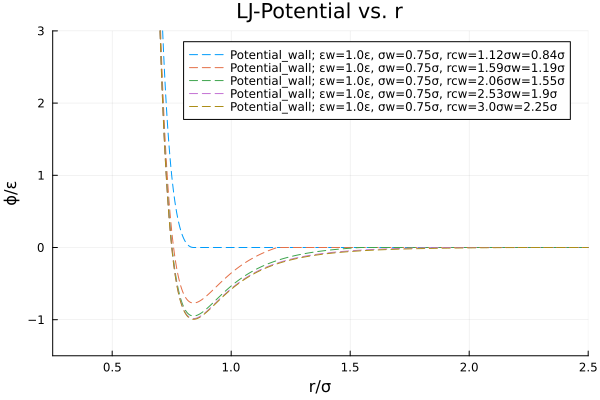
\includegraphics[width=\textwidth]{image/RaRtmap_LJ/LJ-Potential_Rt0.25.png}
      \subcaption{$\text{R}_\text{t}:0.25$}
      \label{}
    \end{minipage} &
    \begin{minipage}[t]{0.2\hsize}
      \centering
      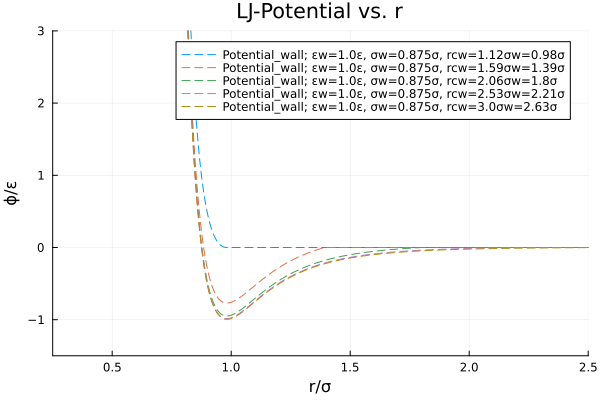
\includegraphics[width=\textwidth]{image/RaRtmap_LJ/LJ-Potential_Rt0.375.png}
      \subcaption{$\text{R}_\text{t}:0.375$}
      \label{}
    \end{minipage} &
    \begin{minipage}[t]{0.2\hsize}
      \centering
      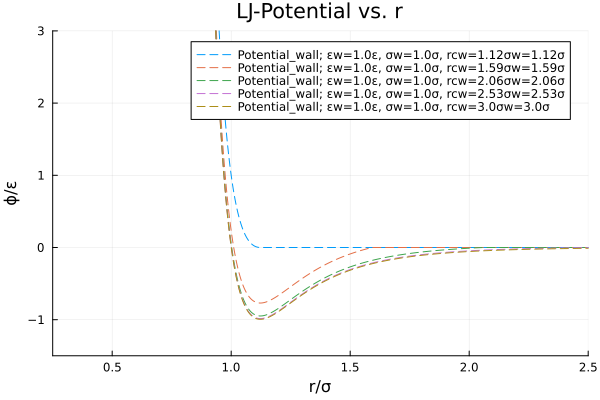
\includegraphics[width=\textwidth]{image/RaRtmap_LJ/LJ-Potential_Rt0.5.png}
      \subcaption{$\text{R}_\text{t}:0.5$}
      \label{}
    \end{minipage} 
  \end{tabular}
  \caption{LJ-potential}
  \label{}
\end{figure}

本章の以降の実験は特記がない限り以下のパラメータで行うものとする. 

\begin{itemize}
  \item $N = 1250$: 粒子数
  \item $\rho {\sigma}^2 = 0.4$: 粒子数密度
  \item $L_x / \sigma = 39.528471 \simeq 39.5$: 系の$x$幅
  \item $L_y / \sigma = 79.0569414 \simeq 79.0$: 系の$y$幅
  \item $k_{\text{B}} T / \varepsilon = 0.43$: 初期温度
  \item $k_{\text{B}} \Delta T / \varepsilon = 0.04$: 熱浴の温度差
  \item $mg\sigma/\varepsilon = 0.0003999718779659611 \simeq 4.0 \times 10^{-4}$: 粒子にかかる重力の大きさ
  \item $\dd t \sqrt{\varepsilon/m{\sigma}^2} = 0.005$: シミュレーションにおける時間刻み.
\end{itemize}

いずれの実験の場合も$t\sqrt{\varepsilon/m{\sigma}^2}=0.0$(シミュレーション開始)の時点では粒子は図\ref{fig:linedUp}のように, 規則正しく並べられている.

\begin{figure}[H]
  \centering
  
\includegraphics[scale=0.2]{image/initial1250.png}
  \caption{$N=1250, t\sqrt{\varepsilon/m{\sigma}^2}=0$}
  \label{fig:linedUp}
\end{figure}

以下に記すのは, シミュレーションについての時間に関して説明するときに用いる文字の説明である.

\begin{itemize}
  \item $t_i \colon$ シミュレーション開始時から, 物理量を解析する際にデータを採用し始める時間. これ以降は定常状態であるとみなす.
  \item $t_f \colon$ シミュレーション開始時から, シミュレーションの終了時までの時間.
\end{itemize}

図 \ref{fig:RaRtmap_time}, 図 \ref{fig:RaRtmap_drop_time}, 図 \ref{fig:dT0_time}, 図 \ref{fig:g0_time}, 図 \ref{fig:RaRtmap10_time}, 図 \ref{fig:qrs10_drop_time}では重心位置の時間発展を示している.

また, 第 \ref{chap:simulation} 章における上記の重心位置の時間発展の図においてはシミュレーション開始時, つまり定常状態とみなすまでの非定常状態の重心位置もグラフに描かれている. しかし, 定常状態であるとみなす時点がわかるように赤い直線を引くことにしている. さらに, 紙面上ではマップ上に並べた画像は小さくなってしまうので, 各系ごとに拡大した画像を最初に示すことにする. 
